\section{گام سوم: پیاده‌سازی حلقه‌ی آموزش و تحلیل همگرایی}

پس از آماده‌سازی داده‌ها و طراحی معماری‌ها، نیازمند یک حلقه‌ی آموزش \lr{(Training Loop)} استاندارد هستیم تا مدل‌ها را بهینه‌سازی کند. در این بخش، فرآیند آموزش برای مدل یادگیری انتقالی \lr{(Transfer Learning)} پیاده‌سازی و تحلیل شده است.

\subsection{تنظیمات آموزش و تابع زیان}
با توجه به اینکه دسته‌بندی روی چندین گروه مختلف انجام می‌شود، از تابع زیان \lr{CrossEntropyLoss} استفاده شد. این تابع به‌طور داخلی عملیات \lr{Softmax} را روی خروجی‌های شبکه اعمال می‌کند و پایداری عددی بالایی دارد. برای به‌روزرسانی وزن‌ها نیز بهینه‌ساز \lr{Adam} با نرخ یادگیری \lr{0.001} به کار رفت. به منظور حفظ وزن‌های از پیش آموزش‌دیده، صرفاً پارامترهای لایه‌ی نهایی به بهینه‌ساز داده شدند.

\begin{tipbox}[معیار ذخیره‌ی بهترین مدل \lr{(Model Checkpointing)}]
برای جلوگیری از نشت اطلاعات، ارزیابی‌ها صرفاً روی داده‌های اعتبارسنجی انجام گرفت و مدلی که بالاترین دقت اعتبارسنجی را در پایان هر دوره داشت، به عنوان بهترین مدل ذخیره شد.
\end{tipbox}

\subsection{تحلیل منحنی‌های آموزش \lr{(Training Curves)}}
مدل به مدت ۵ دوره \lr{(Epoch)} آموزش دید. میانگین زمان هر دوره حدود ۱۲۲ ثانیه ثبت شد و بهترین مدل در دوره‌ی پنجم با دقت \lr{42.44\%} به دست آمد. روند تغییرات خطا و دقت مدل در ادامه رسم شده است.

\begin{figure}[h!]
    \centering
    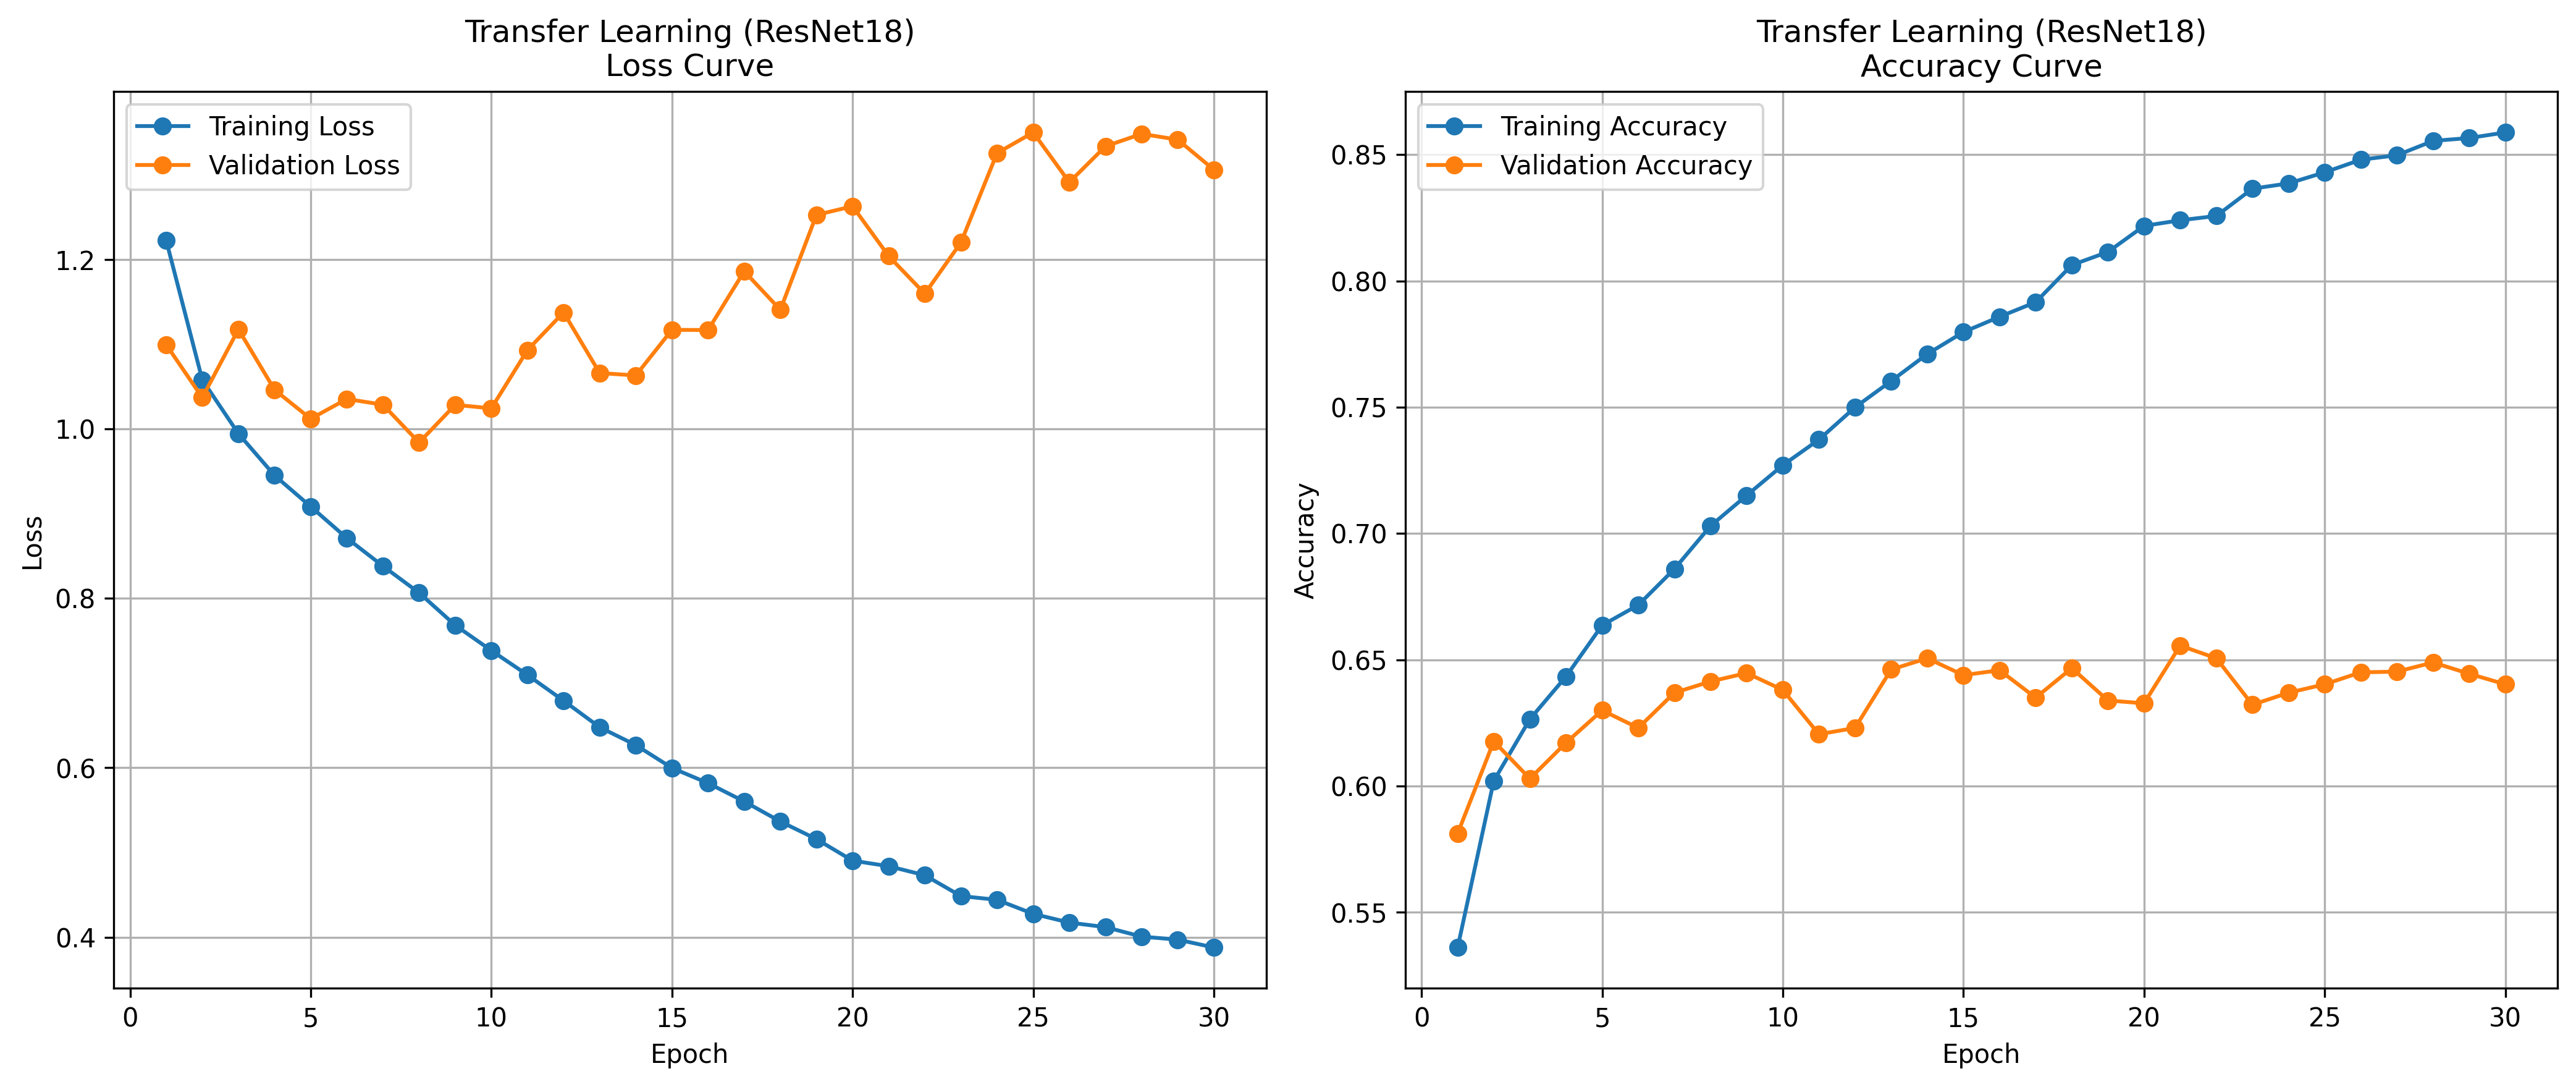
\includegraphics[width=1\textwidth]{images/tl_training_curves.png}
    \caption{منحنی‌های آموزش و اعتبارسنجی برای مدل \lr{ResNet18}}
    \label{fig:tl_curves}
\end{figure}
\newpage
\subsubsection*{تحلیل مشاهدات و پاسخ به پرسش‌های کلیدی:}
با بررسی خروجی‌ها و نمودارها (شکل \ref{fig:tl_curves}) نتایج زیر حاصل می‌شود:
\begin{itemize}
    \item \textbf{وضعیت همگرایی:} دقت از \lr{35.04\%} در دوره‌ی اول به \lr{42.44\%} در دوره‌ی پنجم رسید و خطای آموزش از \lr{1.6430} به \lr{1.4937} کاهش یافت که نشان‌دهنده‌ی همگرایی مناسب مدل است.
    \item \textbf{بررسی بیش‌برازش:} در دوره‌ی پنجم، خطای آموزش (\lr{1.4937}) و خطای اعتبارسنجی (\lr{1.4937}) دقیقاً برابر شدند. همچنین دقت اعتبارسنجی از دقت آموزش مقداری بالاتر قرار گرفت. این رفتار نشان می‌دهد مدل دچار بیش‌برازش \lr{(Overfitting)} نشده است.
    \item \textbf{تحلیل دقت به دست آمده:} با توجه به تعداد کلاس‌ها (دقت حدس تصادفی \lr{14\%})، دستیابی به مقدار \lr{42.44\%} در زمان کوتاه ۵ دوره‌ای مطلوب ارزیابی می‌شود. از آنجا که لایه‌های پایه فریز شده بودند، مدل تنها توانست لایه‌ی طبقه‌بند نهایی را برای ویژگی‌های صورت تنظیم کند.
    \item \textbf{پیشنهاد بهبود:} نمودارها نشان‌دهنده‌ی پتانسیل بالای شبکه برای یادگیری بیشتر هستند. افزایش تعداد دوره‌ها و همچنین آزادسازی لایه‌های استخراج ویژگی در مراحل بعدی، می‌تواند به ارتقای چشمگیر دقت بینجامد.
\end{itemize}